% This text is proprietary.
% It's a part of presentation made by myself.
% It may not used commercial.
% The noncommercial use such as private and study is free
% Sep. 2005 
% Author: Sascha Frank 
% University Freiburg 
% www.informatik.uni-freiburg.de/~frank/
%
% additional usepackage{beamerthemeshadow} is used
%  
%  \beamersetuncovermixins{\opaqueness<1>{25}}{\opaqueness<2->{15}}
%  with this the elements which were coming soon were only hinted
%\documentclass[8pt]{beamer}
\documentclass[10pt]{beamer}
\usepackage{etex}
\newenvironment<>{varblock}[2][\textwidth]{%
  \setlength{\textwidth}{#1}
  \begin{actionenv}#3%
    \def\insertblocktitle{#2}%
    \par%
    \usebeamertemplate{block begin}}
  {\par%
    \usebeamertemplate{block end}%
  \end{actionenv}}
%\usepackage{hyperref}
%\usepackage{natbib}
%\usepackage{beamerthemeshadow}
\usepackage{beamerinnerthemecircles, beamerouterthemeshadow}

\usepackage{amsmath,amssymb,amsfonts}
\usepackage[pdf]{pstricks}
%\usepackage{bbm}
%\usepackage{booktabs}
\usepackage{amsthm}
\usepackage{booktabs}
\usepackage{graphicx}
\usepackage{epsfig}
%\usepackage{graphics}

% MQ: This is to be able to compile on the Riksbank computer. Uncomment with my laptop. Ugly solution but will have to do for now.
%\usepackage{epstopdf}
%\epstopdfsetup{outdir=./}

\usepackage{rotating}

\usepackage{url}
%\usepackage{breqn}
%\usepackage{hyperref}
\usepackage[authoryear]{natbib}
\usepackage{setspace}
\usepackage{multirow}
%\usepackage{harvard}
\usepackage{xcolor}
%\usepackage{multicolumn}
\usepackage{algpseudocode}
\usepackage{sidecap}
\usepackage{bbm} 
\usepackage{courier}
\usepackage{tikz}
\usetikzlibrary{arrows,shapes,snakes,automata,backgrounds,petri}

\tikzset{
  treenode/.style = {align=center, inner sep=0pt, text centered,
    font=\sffamily},
  arn_n/.style = {treenode, circle, white, font=\sffamily\bfseries, draw=black,
    fill=black, text width=1.5em},% arbre rouge noir, noeud noir
  arn_r/.style = {treenode, circle, red, draw=red, 
    text width=1.5em, very thick},% arbre rouge noir, noeud rouge
  arn_x/.style = {treenode, rectangle, draw=black,
    minimum width=0.5em, minimum height=0.5em}% arbre rouge noir, nil
}
\beamertemplatenavigationsymbolsempty

\newenvironment{myenumerate}{\begin{enumerate}[(1)]}{\end{enumerate}} 
\sidecaptionvpos{figure}{c}
% FOR COLORING PARTS  OF TABLE
%\usepackage[beamer,customcolors]{hf-tikz}

%\tikzset{hl/.style={
%    set fill color=red!80!black!40,
%    set border color=red!80!black,
%  },
%}

\mode<presentation> {
    \usetheme{Madrid} %Frankfurt} %Bergen, Berkely, Berlin, Boadilla, CambridgeUS, Darmstadt,
                          %Frankfurt, Goettingen, Singapore, Warsaw
    \usecolortheme{beaver} %seahorse} %default} %beetle, seahorse, wolverine, dolphin, beaver
    %\useoutertheme[subsection=true]{smoothbars} 
    \usefonttheme{default}
    %\usecolortheme{red}
    

	\setbeamercolor{block title}{use=unstructure, fg=white, bg=purple!75!black} %{use=structure,fg=white,bg=purple!75!black}
	%\setbeamercolor{block body}{use=structure,fg=black,bg=white!20!white}    
    %\setbeamercolor{block body}{bg=white}
    \setbeamertemplate{enumerate items}[default]
    \setbeamercolor{enumerate item}{fg=purple!75!black} 
    \setbeamercolor{enumerate subitem}{fg=purple!75!black} 	 
	\setbeamercolor{itemize item}{fg=purple!75!black}  
	\setbeamertemplate{itemize item}[triangle]  
	\setbeamercolor{itemize subitem}{fg=purple!75!black}
	\setbeamertemplate{itemize subitem}[triangle]
	\setbeamertemplate{blocks}[framed]


}



%\usepackage{colortbl}
%\definecolor{yellow}{cmyk}{0,0.18,0.90,0.00}

%\usepackage{xcolor}

%\usepackage[authoryear]{natbib}
\begin{document}
\title[Lecture 5]{Bayesian Learning 732A46: Lecture 5}  
\author[Matias Quiroz]{Matias Quiroz\inst{1}$^{,}$\inst{2}}
\setbeamerfont{institute}{size=\fontsize{7pt}{8pt}}
\institute[LiU and Riksbank]{
  \inst{1}%
   Division of Statistics and Machine Learning, Link\"{o}ping University\\~\\
  \inst{2}%
   Research Division, Sveriges Riksbank\\
     
}

%\institute[Riksbank and LiU]{Sveriges Riksbank and Division of Statistics and Machine Learning, Link\"{o}ping University}

\date[]{April 2016} %\today 

%\usebackgroundtemplate{%
%  \vbox to \paperheight{\vfil\hbox to \paperwidth{\hfil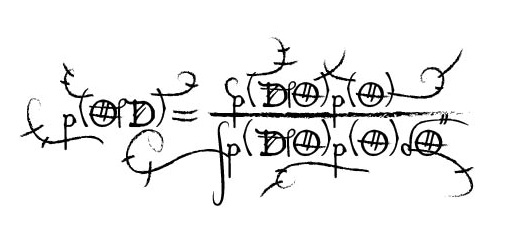
\includegraphics[width=1.5in]{Bayes.jpg}\hfil}\vfil}
%}

{
%\usebackgroundtemplate{\begin{center}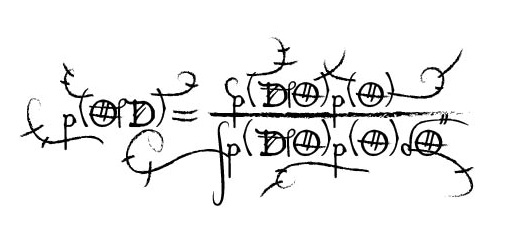
\includegraphics[width=0.4\paperwidth]{Bayes.jpg}\end{center}}
\usebackgroundtemplate{%
  \vbox to \paperheight{\hbox to \paperwidth{\hfil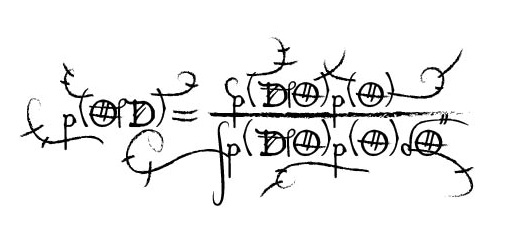
\includegraphics[width=2in]{Bayes.jpg}\hfil}}
}
\begin{frame}
\titlepage
\end{frame}
}
%\frame{\titlepage} 

%\frame{\frametitle{Overview of the talk}\tableofcontents}




\begin{frame}{Lecture overview}

\begin{itemize}
\item The normal model with a conjugate prior for both $\theta, \sigma^2$.
\bigskip
\item Bayesian treatment of the standard linear regression model.
\bigskip
\item 'non-informative' prior + Conjugate prior for the linear model.
\bigskip
\item Shrinkage (regularization/smoothing) through prior distributions. Connection to the frequentist approach.
\bigskip
\item Prediction in the Bayesian linear regression model.

%\item Normal model with conjugate prior
%\item The linear regression model
%\item Non-linear regression
%\item Regularization priors
\end{itemize}
\end{frame}

\begin{frame}{Normal model - conjugate prior for both $\theta$ and $\sigma^2$}

\begin{itemize}
\item \textbf{\color{blue}Model}
\[
y_{1},...,y_{n}|\theta,\sigma^{2}\overset{iid}{\sim}\mathcal{N}(\theta,\sigma^{2})
\]
\bigskip
\item \textbf{\color{blue}Conjugate prior} $\theta,\sigma^2 \sim \mathcal{N}\text{-}Inv\text{-}\chi^{2}(\mu_0, \sigma^2/\kappa_0; \nu_0, \sigma^2_0)$
\begin{gather*}
\theta|\sigma^{2}\sim \mathcal{N}\left(\mu_{0},\frac{\sigma^{2}}{\kappa_{0}}\right)\\
\sigma^{2}\sim Inv\text{-}\chi^{2}(\nu_{0},\sigma_{0}^{2})
\end{gather*}
\bigskip
\item Possible to derive $p(\theta, \sigma^2|y)$ by
\begin{enumerate}
\item Using invaluable techniques {\color{blue}$\#1\text{-}\#3$} from \textbf{\color{blue}Lecture 3}.
\vspace{0.5mm}
\item \textbf{\color{blue}Ignoring} normalizing constants!
\vspace{0.5mm}
\item Having \textbf{\color{red}A LOT} of patience.
\end{enumerate}
\end{itemize}
\end{frame}

\begin{frame}{Normal model - conjugate prior for both $\theta$ and $\sigma^2$, cont.}

\begin{itemize}
\item \textbf{\color{blue}Posterior} $\theta,\sigma^2 |y \sim \mathcal{N}\text{-}Inv\text{-}\chi^{2}(\mu_n, \sigma^2/\kappa_n; \nu_n, \sigma^2_n)$
\begin{gather*}
\theta|\sigma^{2},y \sim \mathcal{N}\left(\mu_{n},\frac{\sigma^{2}}{\kappa_{n}}\right)\\
\sigma^{2}|y\sim Inv\text{-}\chi^{2}(\nu_{n},\sigma_{n}^{2}).
\end{gather*}
where
\begin{eqnarray*}
\mu_{n} & = & \frac{\kappa_{0}}{\kappa_{0}+n}\mu_{0}+\frac{n}{\kappa_{0}+n}\bar{y}\\
\kappa_{n} & = & \kappa_{0}+n\\
\nu_{n} & = & \nu_{0}+n\\
\nu_{n}\sigma_{n}^{2} & = & \nu_{0}\sigma_{0}^{2}+(n-1)s^{2}+\frac{\kappa_{0}n}{\kappa_{0}+n}(\bar{y}-\mu_{0})^{2}.
\end{eqnarray*}

\end{itemize}

\pause{}
\begin{itemize}
\item \textbf{\color{blue}Marginal posterior}
\begin{gather*}
\theta | y\sim t_{\nu_{n}}\left(\mu_{n},\sigma_{n}^{2}/\kappa_{n}\right)...
\end{gather*}
\item ... or just simulate (marginalization by simulation).

\end{itemize}
\end{frame}



\begin{frame}
\frametitle{The standard linear regression model}
\begin{itemize}
\item The model is
\vspace{-5mm}
\begin{eqnarray*}
y_i & = & \beta_1 x_{i1} + \beta_2 x_{i2} + \dots +  \beta_k x_{ik} + \varepsilon_i \\
\varepsilon_i & \sim & \mathcal{N}(0, \sigma^2),
\vspace{-6mm}
\end{eqnarray*}
where $i = 1,\dots,n$. Usually $x_{i1}=1$ for all $i$ [$\beta_1$ is the intercept].
\item \textbf{Parameters} $\theta = (\beta_1, \dots, \beta_k, \sigma^2)^{\prime}$. \textbf{Covariates} $x_i=(1, x_{i2},\dots, x_{ik})^{\prime}$
\item \textbf{\color{blue}Assumptions}
\begin{enumerate}
\item $E[y_i|x_i,\theta] = \beta_1 x_{i1} + \beta_2 x_{i2} + \dots +  \beta_k x_{ik}$ [linear].
\vspace{0.5mm}
\item $V[y_i|x_i,\theta] = \sigma^2$ [homoscedasticity].
\vspace{0.5mm}
\item $y_i|x_i, \theta$ conditionally independent for $i=1,\dots, n$.
\vspace{0.5mm}
\item $\varepsilon_i$ are Normal.
\end{enumerate}
\item \textbf{The notation of}, the posterior distribution $$p(\theta|y)\propto p(y|\theta)p(\theta)$$
omits explicit conditioning. 
\item \textbf{{\color{red}We are implicitly conditioning}} on the $x$'s (covariates) since they are \textbf{non-random}.
\end{itemize}
\end{frame}


\begin{frame}
\frametitle{The standard linear regression model in matrix form}

\begin{itemize}
\item The model in \textbf{\color{blue}matrix form}
\begin{eqnarray*}
\underset{(n \times 1)}{y}  & = & \underset{(n \times k)(k \times 1)}{X\beta} + \underset{(n \times 1)}{\varepsilon}
\end{eqnarray*}
$$y=\begin{bmatrix} y_1 \\ \vdots \\ y_n \end{bmatrix} , \beta = \begin{bmatrix} \beta_1 \\ \vdots \\ \beta_k \end{bmatrix}, \varepsilon=\begin{bmatrix} \varepsilon_1 \\ \vdots \\ \varepsilon_n \end{bmatrix}$$
$$X = \begin{bmatrix} x_1^{\prime} \\ \vdots \\ x_n^{\prime} \end{bmatrix} = \begin{bmatrix} 1 & x_{12} & \dots & x_{1k} \\ \vdots & \vdots & \vdots & \vdots \\ 1 & x_{n2} & \dots & x_{nk} \end{bmatrix} $$
\item \textbf{The likelihood:$\left[ \Sigma = \sigma^2 \underset{(n \times n)}{I} \right]$} $$p(y|\beta, \sigma^2) \propto \left|\Sigma\right|^{-1/2}\exp\left(-\frac{1}{2}\left(y-X\beta\right)^{\prime} \Sigma^{-1}\left(y-X\beta\right)\right) $$ 
\item $\left|\Sigma\right|^{-1/2} = (\sigma^{2n})^{-1/2}=\sigma^{-n}$ and $\Sigma^{-1} = \frac{1}{\sigma^2} I $
\end{itemize}
\end{frame}



\begin{frame}
\frametitle{Normal regression - 'non-informative' prior}
\begin{itemize}
\item The \textbf{standard 'non-informative'} prior $p(\beta, \log(\sigma^2)) \propto c$. 
\bigskip
\item \textbf{Equivalently}: $p(\beta, \sigma^2) \propto \frac{1}{\sigma^2}$.
\bigskip
\item \textbf{\color{blue}Summary}: The posterior is $\mathcal{N}\text{-Inv-}\chi^2(\beta_n, \Sigma_n;\nu_n, s^2_n)$ \\~\\~
\begin{tabular}{ll}
$\beta_n  =  (X^{\prime}X)^{-1} X^{\prime}y $ & $\nu_n = n-k$ \\
$\Sigma_n  =  \sigma^2(X^{\prime}X)^{-1} $ & $s^2_n = \frac{1}{n-k}\left(y-X\beta_n\right)^{\prime} \left(y-X\beta_n\right)$
\end{tabular}
\bigskip
\item \textbf{\color{blue}Simulate} from the joint posterior $p(\beta,\sigma^2|y)$:
\begin{enumerate}
\item $\sigma^2 | y \sim \text{Inv-}\chi^2(\nu_n, s^2_n)$
\item $\beta | \sigma^2, y \sim \mathcal{N}(\beta_n, \Sigma_n).$
\end{enumerate}

\end{itemize}
\end{frame}

\begin{frame}
\frametitle{Normal regression - 'non-informative' prior, cont.}

\begin{itemize}
\item\textbf{\color{blue}Some remarks}
\begin{enumerate}


\item $\beta_n$ is the \textbf{MLE} of $\beta$ in classical statistic [and $s^2_n$ the \textbf{MLE} of $\sigma^2$]. \medskip	
\item We can show that
$$p(\beta|y)=\int p(\beta|\sigma^2,y)p(\sigma^2|y)d\sigma^2 = t_{n-k}(\beta_n, s_n^2(X^{\prime}X)^{-1})$$
\item[] $s_n^2(X^{\prime}X)^{-1}$ - \textbf{standard errors for the MLE} of $\beta$.

\end{enumerate}
\bigskip
\item A Bayesian analysis with a \textit{\color{red}'non-informative prior'} gives the same \textbf{\color{blue}point estimates} as a Frequentist analysis...
%\pause
\bigskip
\item ... but the Bayesian is \textbf{\color{red}richer} - \textbf{knows the whole probability distribution}.
\bigskip
\item I have added slides with the derivation. But I will spare you the pain here.
\end{itemize}

\end{frame}


\begin{frame}
\frametitle{If you dare, do it at home. Nothing but invaluable techniques {\color{blue}$\#1\text{-}\#3$} (and patience!)}
\begin{itemize}
\small{
\item \textbf{Factorize} the posterior ({\color{blue}$\#1$}) 
$$p(\beta, \sigma^2|y) = p(\beta | \sigma^2, y)p(\sigma^2 | y)$$
\item \textbf{Determine first} $p(\beta | \sigma^2, y)$ ({\color{blue}$\#2$}). Use Bayes' theorem and \textbf{\color{blue}treat everything but} $\beta$ \textbf{\color{blue}as proportionality constants}.
\item $p(\beta | \sigma^2, y)= \frac{p(\beta , \sigma^2, y)}{p(\sigma^2, y)} \propto p(y|\beta , \sigma^2) \propto \exp\left(-\frac{1}{2\sigma^2}\left(y-X\beta\right)^{\prime} \left(y-X\beta\right)\right)$
\item A \textbf{\color{blue}quadratic form} in $\beta$. Thus $\beta|\sigma^2, y \sim \mathcal{N}(\beta_n=?, \Sigma_n=?$)
\begin{eqnarray*}
p(\beta|\sigma^2, y) & \propto & \exp\left(-\frac{1}{2}(\beta - \beta_n)^{\prime} \Sigma^{-1}_n (\beta - \beta_n)\right)\\
~ & = & \exp\left(-\frac{1}{2}\left(\beta^{\prime}\Sigma^{-1}_n \beta - 2\beta^{\prime} \Sigma^{-1}_n \beta_n + \beta_n^{\prime}\Sigma^{-1}_n \beta_n \right) \right) \\
~ &  \propto & \exp\left(-\frac{1}{2}\left(\beta^{\prime}\Sigma^{-1}_n \beta - 2\beta^{\prime} \Sigma^{-1}_n \beta_n \right)\right)
\end{eqnarray*}
\item \textbf{Expand} $\exp\left(-\frac{1}{2\sigma^2}\left(y-X\beta\right)^{\prime} \left(y-X\beta\right)\right)$ and \textbf{\color{blue}match terms}.}
\end{itemize}
\end{frame}


\begin{frame}
\frametitle{Derivations, cont.}

\begin{itemize}
\small{
\item \textbf{Expanding}
\begin{eqnarray*}
\exp\left(-\frac{1}{2\sigma^2}\left(y-X\beta\right)^{\prime} \left(y-X\beta\right)\right) & = & \exp\left(-\frac{1}{2\sigma^2}\left(y^{\prime}y-2\beta^{\prime}X^{\prime}y + \beta^{\prime}X^{\prime}X\beta\right)\right) \\
~ & \propto & \exp\left(-\frac{1}{2\sigma^2}\left(\beta^{\prime}X^{\prime}X\beta-2\beta^{\prime}X^{\prime}y\right)\right) 
\end{eqnarray*}
\item \textbf{\color{blue}Match} $\Sigma_n$:
$$\beta^{\prime}X^{\prime}X\beta/\sigma^2=\beta^{\prime}\Sigma^{-1}_n \beta \implies \Sigma^{-1}_n = \frac{1}{\sigma^2}X^{\prime}X \implies \Sigma_n = \sigma^2(X^{\prime}X)^{-1} $$
\item For $\beta_n$, first rewrite
$$2\beta^{\prime}X^{\prime}y/\sigma^2 = 2\beta^{\prime}\underbrace{\Sigma^{-1}_n\Sigma_n}_{I}X^{\prime}y/\sigma^2 $$
\item \textbf{\color{blue}Match} $\beta_n$:
$$2\beta^{\prime}\Sigma^{-1}_n\Sigma_n X^{\prime}y/\sigma^2 = 2\beta^{\prime} \Sigma^{-1}_n \beta_n \implies \beta_n = (X^{\prime}X)^{-1} X^{\prime}y $$}
\end{itemize}
\end{frame}

\begin{frame}
\frametitle{Derivations, cont.}
\begin{itemize}
\item \textbf{We conclude} that $p(\beta|\sigma^2,y)=\mathcal{N}(\beta_n, \Sigma_n$) 
\begin{eqnarray*}
\beta_n & = & (X^{\prime}X)^{-1} X^{\prime}y \\
\Sigma_n & = & \sigma^2(X^{\prime}X)^{-1}.
\end{eqnarray*}
%\textbf{Expanding}
\item Derive $p(\sigma^2|y)$ ({\color{blue}$\#3$}) 
$$p(\sigma^2|y) = \frac{p(\beta, \sigma^2 | y)}{p(\beta|\sigma^2, y)}\propto \frac{p(y|\beta,\sigma^2)p(\sigma^2)}{p(\beta|\sigma^2, y)}$$
\item \textbf{\color{blue}Standard trick}: LHS does not depend on $\beta$ ($\beta$ cancels on RHS).
\item Evaluate RHS using $\beta=\beta_n$ (simplifies the denominator)
\begin{eqnarray*}
\frac{p(y|\beta_n,\sigma^2)p(\sigma^2)}{p(\beta_n|\sigma^2, y)} & \propto & \frac{\sigma^{-n}\exp\left(-\frac{1}{2\sigma^2}\left(y-X\beta_n\right)^{\prime} \left(y-X\beta_n\right)\right)\sigma^{-2}}{\left|\Sigma_n\right|^{-1/2}\exp\left(-\frac{1}{2}\left(\beta_n-\beta_n\right)^{\prime} \Sigma_n^{-1}\left(\beta_n-\beta_n\right)\right)} \\
& = &  \frac{\sigma^{-n}\exp\left(-\frac{1}{2\sigma^2}\left(y-X\beta_n\right)^{\prime} \left(y-X\beta_n\right)\right)\sigma^{-2}}{\left|\Sigma_n\right|^{-1/2}}
\end{eqnarray*}
\end{itemize}
\end{frame}

\begin{frame}
\frametitle{Derivations, cont.}
\begin{itemize}
\item $\left|\Sigma_n\right|=\left|\sigma^{2}(X^{\prime}X)^{-1}\right|=\left|\sigma^{2}I(X^{\prime}X)^{-1}\right|=\overbrace{\left|\sigma^{2}I\right|}^{=\sigma^{2k}}\left|(X^{\prime}X)^{-1}\right|.$
\item Thus $\left|\Sigma_n\right|^{-1/2}=\left(\sigma^{2k}\right)^{-1/2}\left(\left|(X^{\prime}X)^{-1}\right|\right)^{-1/2} \propto \sigma^{-k}$, and
$$p(\sigma^2|y) \propto \sigma^{-n+k-2}\exp\left(-\frac{1}{2\sigma^2}\left(y-X\beta_n\right)^{\prime} \left(y-X\beta_n\right)\right).$$
\item $p(\sigma^2|y) = \text{Inv-}\chi^2(\nu_n, s^2_n)$ if it is \textbf{proportional to}
$$\sigma^{-2(\nu_n/2+1)}\exp\left(-\frac{\nu_n s^2_n}{2\sigma^2}\right).$$
\item \textbf{Rewrite} and \textbf{\color{blue}match terms}
$$p(\sigma^2|y) \propto \sigma^{-2(\overbrace{(n-k)}^{\nu_n}/2+1)}\exp\left(-\frac{\overbrace{n-k}^{\nu_n}}{2\sigma^2}\underbrace{\frac{1}{(n-k)}\left(y-X\beta_n\right)^{\prime} \left(y-X\beta_n\right)}_{s^2_n} \right) $$
\end{itemize}
\end{frame}

\begin{frame}
\frametitle{Derivations, \textbf{\color{blue}final slide}!}
\begin{itemize}
\item \textbf{\color{blue}We have proven} that the posterior is $\mathcal{N}\text{-Inv-}\chi^2(\beta_n, \Sigma_n;\nu_n, s^2_n)$ \\~\\~
\begin{tabular}{ll}
$\beta_n  =  (X^{\prime}X)^{-1} X^{\prime}y $ & $\nu_n = n-k$ \\
$\Sigma_n  =  \sigma^2(X^{\prime}X)^{-1} $ & $s^2_n = \frac{1}{n-k}\left(y-X\beta_n\right)^{\prime} \left(y-X\beta_n\right)$
\end{tabular}
\end{itemize}
\end{frame}




\begin{frame}
\frametitle{Normal regression - Conjugate prior for $\beta,\sigma^2$}
\begin{itemize}
\item An informative prior is helpful for \textbf{\color{blue}model regularization}. 
\item \textbf{\color{blue}Conjugate prior} $p(\beta, \sigma^2) = \mathcal{N}\text{-Inv-}\chi^2(\beta_0, \sigma^2 \Omega^{-1}_0;\nu_0, s^2_0)$,
\begin{eqnarray*}
p(\beta|\sigma^2) & = & \mathcal{N}(\beta_0, \sigma^2 \Omega^{-1}_0)\\
p(\sigma^2) & = & \text{Inv-}\chi^2(\nu_0, s^2_0)
\end{eqnarray*}
\item The role of the \textbf{hyperparameters} in the prior.
\begin{itemize}
\item[(1)] $\beta_0$ - the mean. $\beta_0 = 0$ common choice.
\item[(2)] $\Omega_0$ - the "precision". Common choice $\Omega_0 = \lambda I$ [$\Omega_0^{-1} = \frac{1}{\lambda} I$]. \\ \textbf{Larger $\lambda \implies$ {\color{blue}prior concentrates more} around $\beta_0$}. 
We can even have
$$\Omega_0=\text{diag}(\lambda_1, \dots, \lambda_k).$$
\item[(3)] $\nu_0$ - prior degrees of freedom.
\item[(4)] $s^2_0$ - prior average sum of squares.
\end{itemize}
\item With $\beta_0=0$, {\color{purple!75!black}(2)} is an example of \textbf{model regularization through the prior}. Tackles \textbf{\color{red}over-fitting problems} that occur in models with many parameters.
\end{itemize}
\end{frame}

\begin{frame}
\frametitle{The posterior with the conjugate prior for $\beta,\sigma^2$}
\begin{itemize}
\item \textbf{\color{red}Tedious} algebra with 'non-informative' prior. 
\medskip
\item A \textbf{\color{red}nightmare} here - \textbf{but still only} {invaluable techniques \color{blue}$\#1\text{-}\#3$}.
\medskip
\item \textbf{It's form:} a matrix version of the normal model with a conjugate on $\theta, \sigma^2$.
\medskip
\item Let $\hat{\beta}=(X^{\prime}X)^{-1}X^{\prime}y$ [\textbf{'Non-informative'} case, \textbf{MLE}].
\medskip
\item \textbf{The posterior} $p(\beta,\sigma^2|y)=p(\beta|\sigma^2,y)p(\sigma^2|y)$
\begin{eqnarray*}
p(\beta|\sigma^2,y) & = & \mathcal{N}(\beta_n, \sigma^2 \Omega^{-1}_n)\\
p(\sigma^2|y) & = & \text{Inv-}\chi^2(\nu_n, s^2_n)
\end{eqnarray*}
\begin{tabular}{ll}
$\beta_n  =  (X^{\prime}X+\Omega_0)^{-1}(X^{\prime}X\hat{\beta} + \Omega_0 \beta_0)  $ & $\Omega_n = X^{\prime}X+\Omega_0 $ \\
$\nu_n = \nu_0 + n $ & $\nu_n s^2_n = \nu_0s^2_0+y^{\prime}y+\beta_0^{\prime}\Omega_0 \beta_0 - \beta_n^{\prime}\Omega_n \beta_n$
\end{tabular}
\medskip
\item \textbf{\color{blue}Note}: the posterior mean is a weighted average of data and prior information.
\end{itemize}
\end{frame}


\begin{frame}
\frametitle{Shrinkage illustration with the conjugate prior for $\beta,\sigma^2$}
\begin{itemize}

\item \textbf{\color{blue}Shrinkage illustration}:\vspace{2mm}\\ With $X^{\prime}X = I$ and $p(\beta|\sigma^2)=\mathcal{N}(\beta_0, \sigma^2/\lambda I)$ [$\Omega_0 = \lambda I$]
$$\beta_n  =  (I+\lambda I)^{-1}(I\hat{\beta} + \lambda I \beta_0)= \overbrace{\frac{1}{1+\lambda}}^{0<w_1<1}\hat{\beta} + \overbrace{\frac{\lambda}{1+\lambda}}^{0<w_2<1}\beta_0 \quad [w_1+w_2=1].$$
%\bigskip
\item \textbf{\color{red}Note that} 
\begin{enumerate}
\item $\lambda \rightarrow 0 \implies \beta_n \rightarrow \hat{\beta}$.
\item $\lambda \rightarrow \infty \implies \beta_n \rightarrow \beta_0$.
\end{enumerate}
\medskip
%\pause
\item \textbf{\color{red}'Non-informative' priors} [$\lambda = 0$] \textbf{\color{red}do not shrink}!... 
\medskip
\item ... \textbf{Neither does {\color{red}Frequentist} {\color{blue}OLS} nor {\color{blue}MLE} estimates!} 

\end{itemize}
\end{frame}

\begin{frame}{Example: {\color{blue}Bayesian spline} with shrinkage prior}


\begin{center}
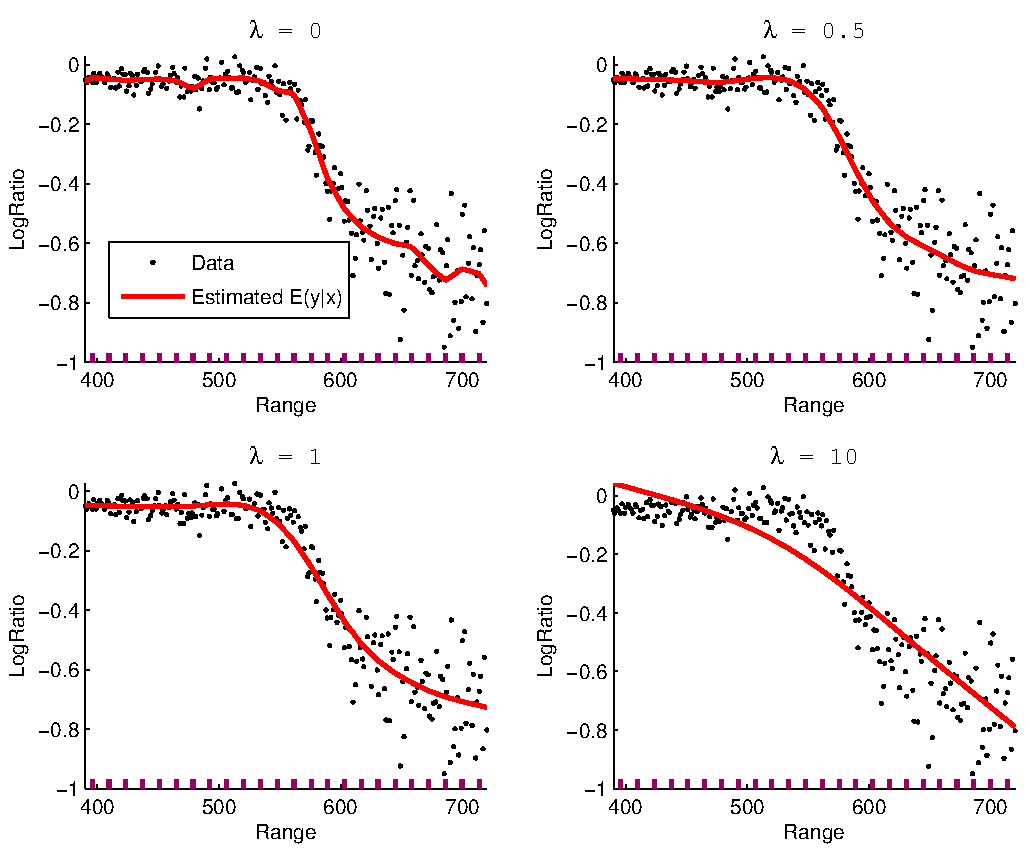
\includegraphics[scale=0.55]{LidarPoly1Knots24}
\par\end{center}

\end{frame}


\begin{frame}
\frametitle{Polynomial regression as a simple linear regression}
\begin{itemize}
\item Consider only a \textbf{single covariate} for simplicity.
\item A general regression model with \textbf{additive noise} 
$$y_i = f(x_i;\beta) + \varepsilon_i, \quad \varepsilon_i \sim \mathcal{N}(0, \sigma^2).$$
\item \textbf{\color{blue}Polynomial regression}
\begin{itemize}
\item $f(x_i;\beta) = \beta_0 + \beta_1 x_i$ - linear regression 
\item $f(x_i;\beta) = \beta_0 + \beta_1 x_i + \beta_2 x_i^2$  - quadratic regression 
\item $f(x_i;\beta) = \beta_0 + \beta_1 x_i + \dots + \beta_p x_i^p$ - polynomial order $p$.
\end{itemize}
\begin{center}
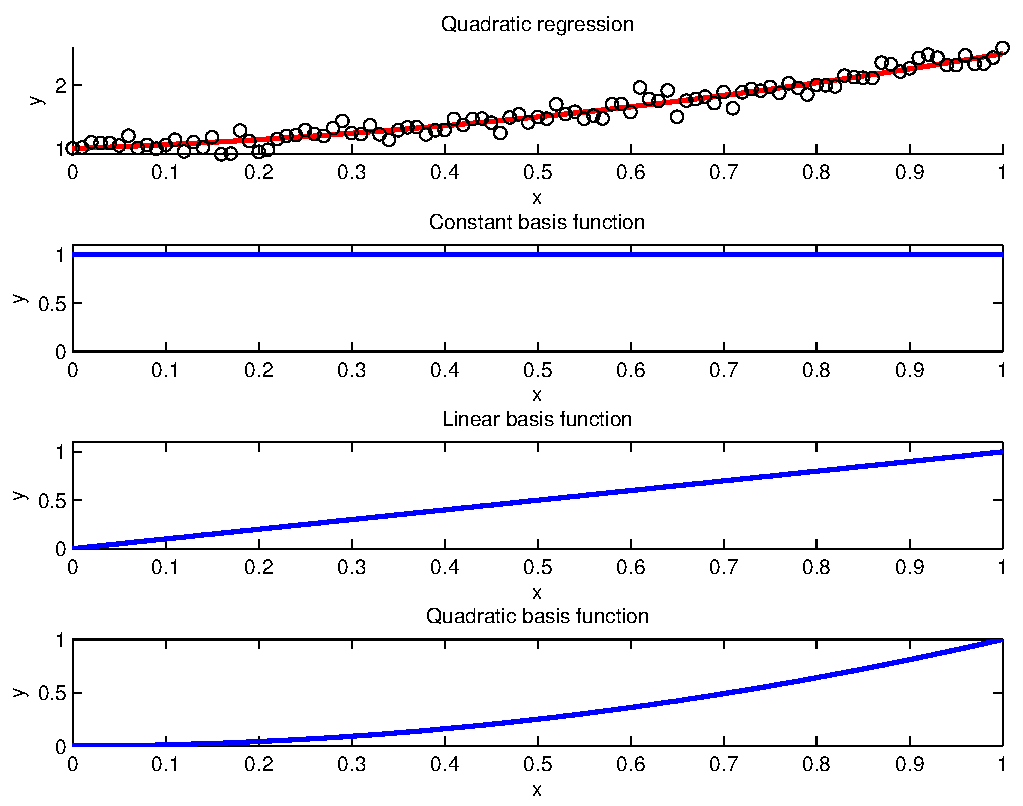
\includegraphics[scale=0.35]{quadraticBasis}
\par\end{center}

\end{itemize}
\end{frame}


\begin{frame}
\frametitle{Polynomial regression as a simple linear regression, cont.}
\begin{itemize}
\item \textbf{Can be written}
$$y = X_p \beta + \varepsilon, \quad X_p = (1,x,x^2,\dots x^p)  \in n \times (p+1).$$
\smallskip
\item $x$ is \textbf{\color{blue}basis expanded} $X_p = (h_0(x),h_1(x),h_2(x),\dots h_p(x))$ where $$h_j(x)=x^j,\quad j=1,\dots,p, \text{ are the {\color{blue}basis functions}}.$$
\smallskip
\item \textbf{Note:} The model is \textbf{Non-linear} in data but \textbf{\color{blue}still linear in parameter}
\bigskip

\item Estimation as before but with $X_p$ in place of $X$.
\bigskip
\item \textbf{Problem:} Polynomials are \textbf{\color{red}too global} - fit becomes unstable. 
%\item A spline model augments the predictors $X$ with "local polynomials" also known as local basis functions.
\end{itemize}
\end{frame}




\begin{frame}
\frametitle{Shrinkage in a spline regression model}
\begin{itemize}
\item \textbf{Splines} to the rescue! Like polynomials but \textbf{\color{blue}more local}.
\item \textbf{Example:} Truncated \textit{power splines}. Basis functions
$$h_j(x) = \begin{cases} (x-\xi_j)^a \quad \quad \text{if }x>\xi_j \\ ~~~~~ 0 \quad \quad \quad~~ \text{otherwise}. \end{cases},$$
where $\xi_j$ ($j=1,\dots,p)$ are the \textbf{\color{blue}knots} which are given.
\begin{center}
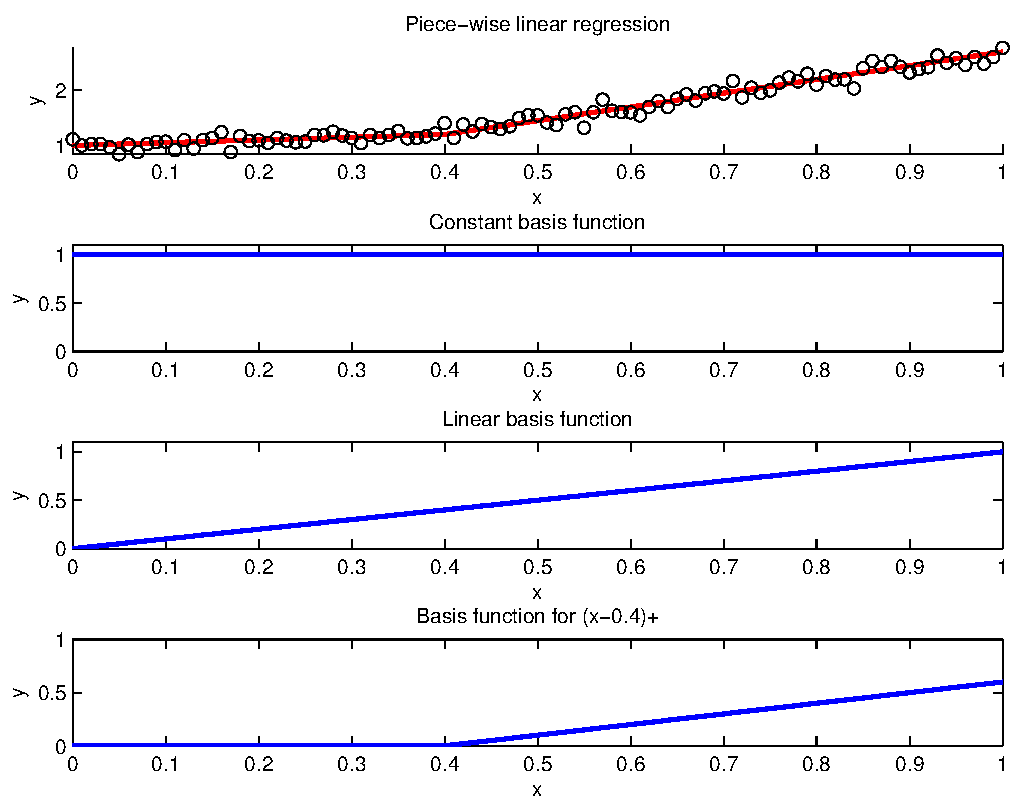
\includegraphics[scale=0.4]{brokenStickBasis}
\par\end{center}

\end{itemize}
\end{frame}



\begin{frame}
\frametitle{Shrinkage in a spline regression model}
\begin{itemize}

\item \textbf{\color{blue}Note}: given the knots, the \textbf{spline regression model}
is a linear regression of $y$ on the basis expanded matrix $$X_p = (1,x ,h_1(x),\dots h_p(x))$$
(common to include \textbf{an intercept} + \textbf{a linear basis} function).
\medskip
\item Estimation as in the linear regression. Just change $X$ for $X_p$.
\medskip
\item Typically many knots. \textbf{Regularization} required for a smooth fit.
\medskip
\item \textbf{\color{blue}Let's see the figure again}! 
\end{itemize}
\end{frame}



\begin{frame}
\frametitle{Shrinkage in Bayesian spline (note the {\color{blue}knots}!)}
\begin{figure}[H]
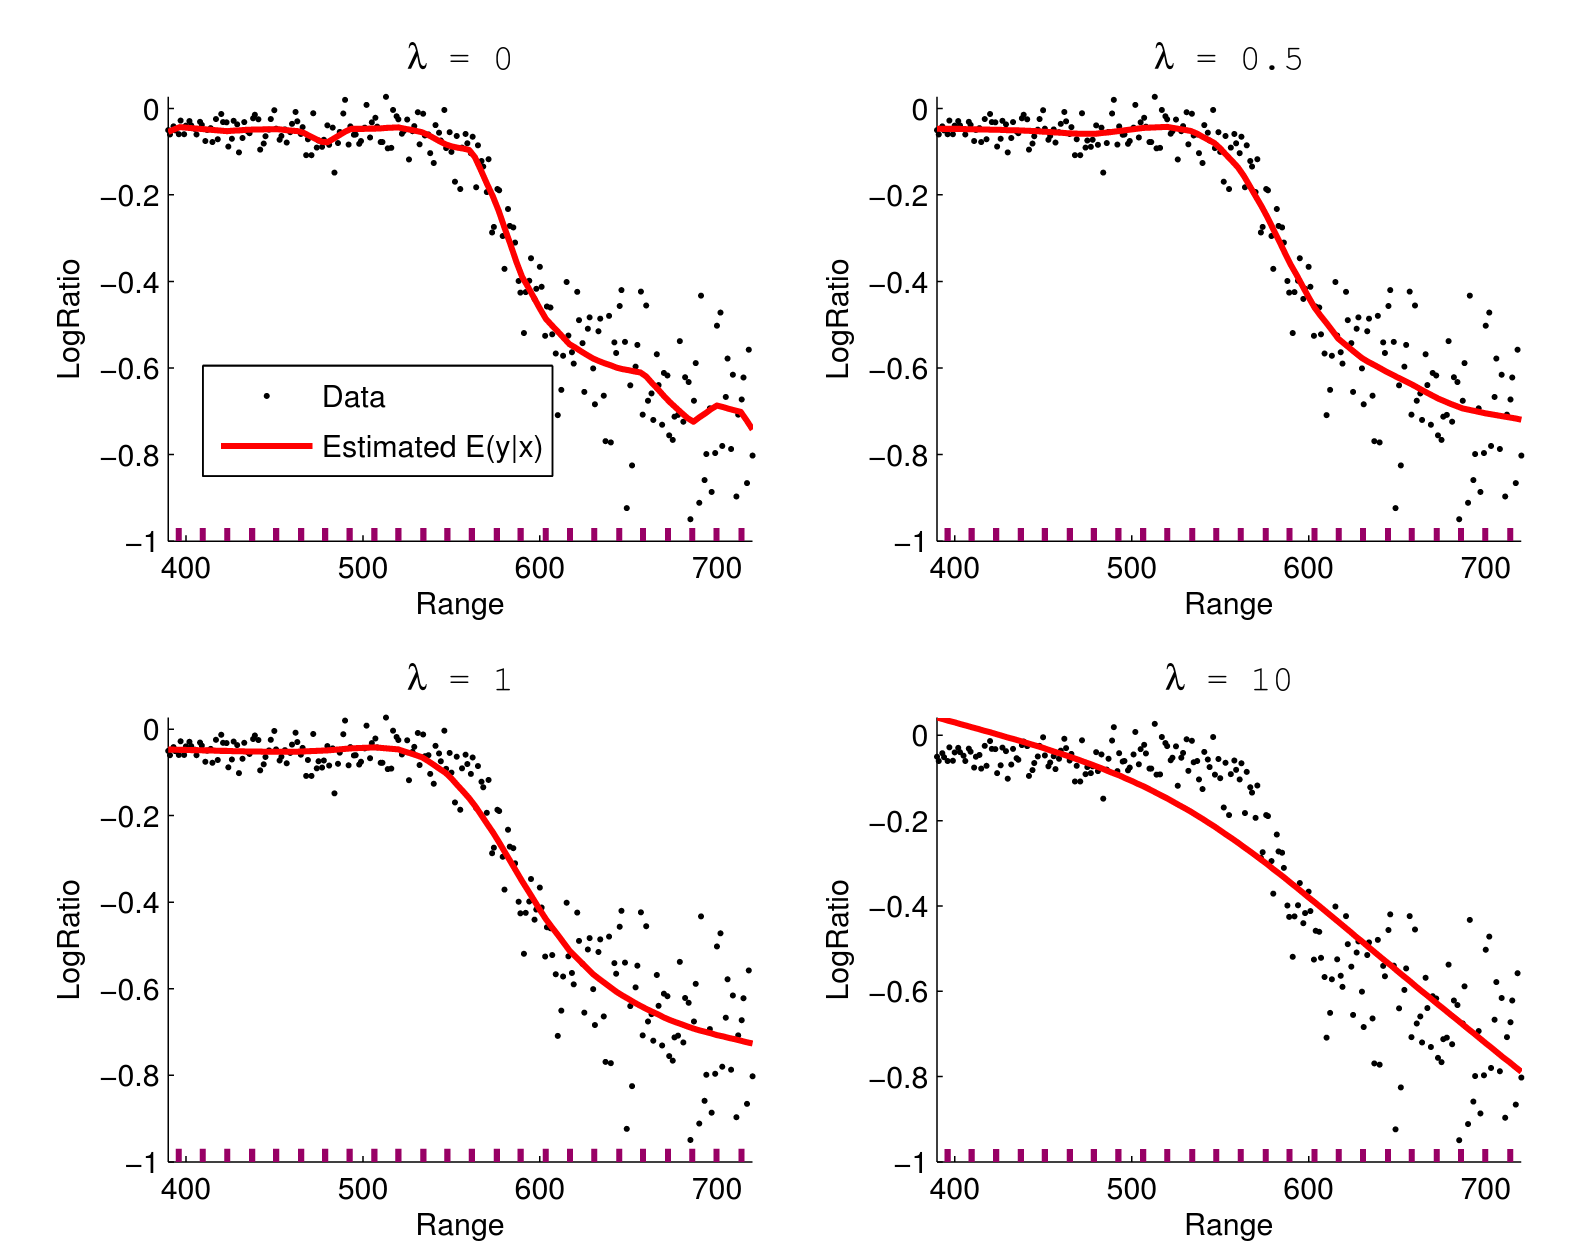
\includegraphics[width=0.8\columnwidth]{SplineFit}
%\protect\caption{LIDAR data.}
\end{figure}
\end{frame}




\begin{frame}
\frametitle{Shrinkage: Frequentist vs Bayesian}
\begin{itemize}
\item Frequentists instead shrink by minimizing a \textbf{\color{blue}penalized} RSS.
\item Residual Sum of Squares (RSS): $$\mathrm{RSS}(\beta)=(y - f(X;\beta))^{\prime}(y - f(X;\beta)).$$
\item Example \textbf{\color{blue}ridge regression}:
$$\hat{\beta}_{ridge} = \arg \min_{\beta} RSS(\beta) + \lambda \beta^{\prime}\beta \longrightarrow \hat{\beta}_{ridge} = (X^{\prime}X+\lambda I)^{-1}X^{\prime}y$$
\item The same as the \textbf{\color{blue}Bayesian posterior mean} $\beta_n$ we have derived with $\beta_0=0$ and $\Omega_0=\lambda I$...
\pause
\item ... the frequentists are indeed using "prior information"... \textbf{\color{red}but they are hiding it}! 
\item The Bayesian shrinkage prior is \textbf{\color{blue}interpretable}. Nothing ad hoc.
\end{itemize}
\end{frame}


\begin{frame}
\frametitle{Other Shrinkage priors}
\begin{itemize}
\item Other shrinkage priors can be used but they are \textbf{not conjugate}.
\medskip
\item MCMC methods can be used for estimation.
\medskip
\item The famous frequentist \textbf{\color{blue}Lasso variable selection} method is equivalent to \textbf{the posterior mode} using the prior $$p(\beta_k|\sigma^2) = \frac{\lambda}{2\sigma^2} \exp\left(-\lambda \frac{|\beta_k|}{\sigma^2}\right) \quad \left[\mathrm{Laplace}\left(0, \frac{\sigma^2}{\lambda}\right)\right].$$
\medskip
\item Laplace distribution - \textbf{heavy tails}.
\medskip
\item \textbf{\color{blue}Laplace prior}: many $\beta_{k}$ are close to zero, but some $\beta_{i}$
may be very large.
\medskip
\item Normal distribution - \textbf{light tails}. 
\medskip
\item \textbf{\color{blue}Normal prior}: most $\beta_{k}$ are fairly equal in size, and no single $\beta_{k}$ can be very much larger than the other ones.


\end{itemize}
\end{frame}

\begin{frame}
\frametitle{Estimating the shrinkage parameter $\lambda$ from the data}
\begin{itemize}
\item So far implicitly assumed that $\lambda$ \textbf{is known}.
\medskip
\item Crossvalidation is one possibility. But this \textbf{\color{red}is not} a Bayesian solution.
\medskip
\item \textbf{\color{blue}Question}: What would a Bayesian solution be?
\medskip
\pause
\item \textbf{\color{blue}Clue}: Bayesians treat \textit{any} \textbf{unknown quantity} as...
\pause
\medskip
\item ... a \textbf{\color{blue}random variable}!
\medskip
\item Treat $\lambda$ as a r.v. Inference through $p(\beta,\sigma^2,\lambda|y)$
\medskip
\item Assign a prior $p(\lambda)$ and derive $p(\lambda|y)$.

%$$p(\lambda|y) \propto \left(\frac{}{}\right $$
\end{itemize}
\end{frame}

\begin{frame}
\frametitle{Estimating the shrinkage parameter $\lambda$ from the data,cont.}
\begin{itemize}
\item The \textbf{joint posterior} factorizes ({\color{blue}$\#1$}) $$p(\beta,\sigma^2,\lambda|y) = p(\beta|\sigma^2,\lambda,y)p(\sigma^2|\lambda,y)p(\lambda|y),$$ where ({\color{blue}$\#1\text{-}\#2$} to derive)
\\~\\
\begin{tabular}{rcl}
$\textbf{\color{blue}Prior} \quad\quad\quad$ &  $\rightarrow$ & 
\vspace{3mm}
$\quad\quad\quad\textbf{\color{blue}Posterior}$ \\
\vspace{3mm}
$\beta | \sigma^2, \lambda \sim \mathcal{N}(0,\sigma^2\Omega_0^{-1})$ & $\rightarrow$ & $\beta|\sigma^2, \lambda, y \sim  \mathcal{N}(\beta_n, \sigma^2\Omega_n^{-1})$ \\
\vspace{2mm}
$\sigma^2 \sim \text{Inv-}\chi^2(\nu_0,s_0^2)$ & $\rightarrow$ & $\sigma^2 | \lambda, y \sim \text{Inv-}\chi^2(\nu_n,s_n^2)$ \\
$\lambda \sim p(\lambda)$ & $\rightarrow$ & $\lambda| y \sim  \sqrt{\frac{|\Omega_0 |}{|\Omega_n |}}\left(\frac{\nu_ns^2_n}{2}\right)^{-\nu_n/2} p(\lambda)$
%$p(\sigma^2)$ & $=$ & $\text{Inv-}\chi^2(\nu_0,s_0^2)$ & $\rightarrow$ & $p(\sigma^2|\lambda,y)$ & $=$ &$ \text{Inv-}\chi^2(\nu_n,s_n^2)$ \\~\\
%$p(\sigma^2)$ & $=$ & $\text{Inv-}\chi^2(\nu_0,s_0^2)$ & $\rightarrow$ & $p(\sigma^2|\lambda,y)$ & $=$ &$ \sqrt{\frac{|\Omega_0 |}{|\Omega_n |}}\left(\frac{\nu_ns^2_n}{2}\right)^{-\nu_n/2} p(\lambda)$
\end{tabular}
\\~\\ and \\~\\
\begin{tabular}{ll}
$\beta_n  =  (X^{\prime}X+\Omega_0)^{-1}X^{\prime}y  $ & $\Omega_n = X^{\prime}X+\Omega_0 $ \\
$\nu_n = \nu_0 + n $ & $\nu_n s^2_n = \nu_0s^2_0+y^{\prime}y - \beta_n^{\prime}\Omega_n \beta_n$
\end{tabular}
%$$p(\lambda|y) \propto \left(\frac{}{}\right $$
\end{itemize}
\end{frame}



\begin{frame}
\frametitle{Prediction in linear regression}
\begin{itemize}
\item \textbf{Predict the outcome} $\tilde{y}$ for a set of observations with covariates $\tilde{X}$ 
\medskip
\item \textbf{\color{blue}Posterior predictive density} [implicitly conditioning on $X$ and $\tilde{X}$]
\begin{eqnarray*}
p(\tilde{y}|y) & = & \int_{\sigma^2} \int_{\beta} p(\tilde{y}|y, \beta, \sigma^2)p(\beta, \sigma^2 |y) d\beta d\sigma^2 \\
 ~ & = &  \int \int p(\tilde{y}|\beta, \sigma^2)p(\beta,\sigma^2|y) d\beta d\sigma^2
\end{eqnarray*}
if $\tilde{y}$ and $y$ are conditionally independent (given $\beta,\sigma^2$).
\medskip
\item \textbf{We can simulate} from $p(\tilde{y}|y)$ by
\begin{enumerate}
\item $\beta, \sigma^2 \sim p(\beta,\sigma^2|y)$
\vspace{2mm}
\item $\tilde{y}|\beta, \sigma^2 \sim p(\tilde{y}|\beta,\sigma^2)=\mathcal{N}(\tilde{X}\beta, \sigma^2 I).$
\end{enumerate}
\medskip
\item {\color{purple!75!black}Step 1.}: First $\sigma^2$ and then $\beta|\sigma^2$ $\left[p(\beta,\sigma^2|y)= p(\beta|\sigma^2,y)p(\sigma^2|y)\right]$.
\medskip
\item If the \textbf{shrinkage $\lambda$ is estimated} use $p(\beta,\sigma^2, \lambda|y)$ instead.
\end{itemize}
\end{frame}



\end{document}

